\documentclass{article}
\usepackage[T1]{fontenc}
\usepackage[polish]{babel}
\usepackage[utf8]{inputenc}
\usepackage[table,xcdraw]{xcolor}
\usepackage[normalem]{ulem}
\usepackage{lmodern}
\usepackage{fullpage}
\usepackage{longtable}
\usepackage{tikz}
\usetikzlibrary{shapes,arrows,positioning}
\selectlanguage{polish}


\begin{document}
\begin{center}
\textbf{Projekt Zespołowy - Projekt zarządzania ryzykiem}
\end{center}
\mbox{}\\
\paragraph{Planowanie zarządzania ryzykiem}
\mbox{}\\

Ryzyko to prawdopodobieństwo wystąpienia sytuacji, która może oddziaływać na dalszy przebieg projektu- jego jakość, zakres, koszty i/lub harmonogram.
Zarządzanie ryzykiem jest bardzo ważnym elementem każdego projektu, które polega na monitorowaniu i obniżaniu ryzyka projektu do poziomu akceptowalnego przez menadżera projektu.
W planie zarządzania projektem należy zdefiniować wstępną ocenę skutków wystąpienia ryzyka, oraz wstępną ocenę prawdopodobieństwa wystąpienia takiego zdarzenia.
\mbox{}\\

Wstępna ocena skutków wystąpienia ryzyka – wstępna ocena skutków wystąpienia danego ryzyka została sklasyfikowana opisowo, według następującego klucza:
\begin{itemize}
\item{Niskie}
\item{Średnie}
\item{Wysokie}
\end{itemize}

Wstępna ocena prawdopodobieństwa – wstępna ocena skutków wystąpienia danego ryzyka została sklasyfikowana opisowo, według następującego klucza:
\begin{itemize}
\item{Mało prawdopodobne (0 – 20\%)}
\item{Możliwe (20\% - 60\%)}
\item{Prawdopodobne (60\% - 100\%)}
\end{itemize}


Każdy z członków zespołu odpowiedzialny jest za kontrolę i dbałość o jakość projektu, w celu uniknięcia wystąpienia ryzyka.  
Na każdym z etapów projektu należy przeprowadzić kontrolę ryzyka, poprzez porównanie wyników prac z możliwymi przypadkami zdefiniowanymi w formularzach analizy ryzyka, należy zwrócić uwagę również na inne, nie ujęte w formularzach sytuację, i w razie stwierdzenia, że jest to sytuacja zidentyfikowana jako ryzyko, należy po uzgodnieniu z liderem projektu zaktualizować lub dodać kolejny formularz analizy ryzyka. 
Progi akceptacji czyli kryteria określające, kiedy powinny zostać podjęte działania będące odpowiedzią na zaistniałe ryzyko, ustalane są przez wszystkich członków zespołu.

\paragraph{Identyfikacja ryzyka}
\mbox{}\\

W procesie tym występuje wykrycie źródeł ryzyka, a następnie ich usystematyzowanie według przyjętych kategorii. Po przeprowadzeniu analizy, zostały stworzone następujące kategorie źródeł ryzyka:

\begin{enumerate}
\item{Strategiczne i handlowe}
	\begin{enumerate}
		\item{Dodawanie nowych wymagań po zamknięciu specyfikacji}
		\item{Nieczytelność serwisu}
	\end{enumerate}
\item{Ekonomiczne, finansowe i rynkowe}
	\begin{enumerate}
		\item{Niemożność ukończenia projektu ze względu na brak finansów}
	\end{enumerate}
\item{Organizacyjne, zarządzania i związane z czynnikiem ludzkim}
	\begin{enumerate}
		\item{Błędnie stworzona specyfikacja systemu}
		\item{Utrudnienia w komunikacji}
		\item{Choroby, wypadki}
		\item{Niedoświadczony zespół}
		\item{Nieodpowiedni kierownik zespołu}
	\end{enumerate}
\item{Techniczne, operacyjne i związane z infrastrukturą}
	\begin{enumerate}
		\item{Utrata danych}
		\item{Wybór nieodpowiednich technologii do realizacji systemu}
		\item{Błędy w implementacji systemu}
	\end{enumerate}
\end{enumerate}

\paragraph{Jakościowa analiza ryzyka} \mbox{}\\

Analiza skutków wystąpienia ryzyka, w kolejności od krytycznych do mających najmniejszy wpływ na projekt:
\begin{enumerate}
\item{Utrata danych}
\item{Błędnie stworzona specyfikacja projektu}
\item{Dodawanie nowych wymagań po zamknięciu specyfikacji}
\item{Wybór nieodpowiednich technologii do realizacji systemu}
\item{Błędy w implementacji systemu}
\item{Choroby/wypadki}
\item{Niedoświadczony zespół}
\item{Nieodpowiedni kierownik zespołu}
\item{Niemożność ukończenia projektu ze względu na brak finansów}
\item{Utrudnienia w komunikacji}
\item{Nieczytelność serwisu}
\end{enumerate}

Macierz ryzyka, redukcja grup, przypisanie do formularzy, ew. Symptomy

\paragraph{Ilościowa analiza ryzyka} \mbox{}\\

Oszacowanie wagi dla każdego ryzyka na podstawie prawdopodobieństwa wystąpienia, oraz wpływu na projektu
Obliczane według następującego wzoru (skutek\_ryzyka \* prawd\_wystąpienia)
\mbox{}\\\mbox{}\\

Wagi dla skutków ryzyka
\begin{itemize}
\item{Niskie     - Waga: 1}
\item{Średnie    - Waga: 2}
\item{Wysokie	 - Waga: 3}
\end{itemize}
\mbox{}\\
\mbox{}\\\mbox{}\\

Wagi dla prawdopodobieństw wystąpienia
\begin{itemize}
\item{Mało prawdopodobne (0 – 20\%) - Waga: 1}
\item{Możliwe (pow. 20\% - 60\%) - Waga: 2}
\item{Prawdopodobne (pow. 60\% - 100\%) - Waga: 3}
\end{itemize}
\mbox{}\\ \mbox{}\\

Źródła ryzyka wraz z wagami prezentują się następująco:
\begin{enumerate}
\item{Utrata danych - (3*2) = 6}
\item{Błędnie stworzona specyfikacja projektu - (3*2) = 6}
\item{Dodawanie nowych wymagań po zamknięciu specyfikacji - (3*1) = 3}
\item{Wybór nieodpowiednich technologii do realizacji systemu - (3*2) = 6}
\item{Błędy w implementacji systemu - (3*2) = 6}
\item{Choroby/wypadki - (3*1) = 3}
\item{Niedoświadczony zespół - (3*2) = 6}
\item{Nieodpowiedni kierownik zespołu - (3*1) = 3}
\item{Niemożność ukończenia projektu ze względu na brak finansów - (3*1) = 3}
\item{Utrudnienia w komunikacji - (1*1) = 1}
\item{Nieczytelność serwisu - (1*1) = 1}
\end{enumerate}
\mbox{}\\ \mbox{}\\\mbox{}\\\mbox{}\\\mbox{}\\\mbox{}\\\mbox{}\\ \mbox{}\\ \mbox{}\\\mbox{}\\

\paragraph{Planowanie reakcji na ryzyko}
\mbox{}\\ \mbox{}\\
%\begin{table}[]
%\centering
%\caption{My caption}
\hspace*{-0.9cm}
\label{my-label}
\begin{tabular}{|l|l|l|}
\hline
\rowcolor[HTML]{C0C0C0} 
Zagrożenie                                                                                            & Strategia  & Środki zaradcze                                                                                                                                                                                                                         \\ \hline
\begin{tabular}[c]{@{}l@{}}Dodawanie nowych wymagań po\\ zamknięciu specyfikacji\end{tabular}         & Redukcja   & \begin{tabular}[c]{@{}l@{}}Upewnienie się, że lista wymagań  jest kompletna jeszcze przed\\  zamknięciem specyfikacji\end{tabular}                                                                                                       \\ \hline
Nieczytelność serwisu                                                                                 & Redukcja   & Konsultacje z klientem, w celu akceptacji wyglądu aplikacji                                                                                                                                                                             \\ \hline
\begin{tabular}[c]{@{}l@{}}Niemożność ukończenia projektu ze \\ względu na brak finansów\end{tabular} & Redukcja   & \begin{tabular}[c]{@{}l@{}}Przeanalizowanie serwisów, w celu znalezienia najtańszego\\  lub darmowego rozwiązania\end{tabular}                                                                                                          \\ \hline
Błędnie stworzona specyfikacja systemu                                                                & Redukcja   & \begin{tabular}[c]{@{}l@{}}Konsultacje z ekspertem ze strony klienta,  konsultacje\\ z osobami doświadczonymi w temacie projektu, udzielanie\\  się na forach dyskusyjnych, związanych  z używaną\\ w systemie technologią\end{tabular} \\ \hline
Utrudnienia w komunikacji                                                                             & Redukcja   & Zapewnienie nadmiarowej ilości kanałów komunikacyjnych                                                                                                                                                                                  \\ \hline
Choroby, wypadki                                                                                      & Akceptacja & \begin{tabular}[c]{@{}l@{}}Każdy członek zespołu powinien być samodzielny, by być\\  w stanie przejąć obowiązki i zadania  od innego członka zespołu.\end{tabular}    \\ \hline
Niedoświadczony zespół                                                                                & Redukcja   & \begin{tabular}[c]{@{}l@{}}Przeprowadzenie szkolenia przez eksperta z danej technologii,\\   samokształcenie się przez wszystkich członków zespołu\\   z oficjalnej dokumentacji\end{tabular}                                             \\ \hline
Nieodpowiedni kierownik zespołu                                                                       & Redukcja   & \begin{tabular}[c]{@{}l@{}}Sprawdzenie kompetencji osoby, która ma zostać kierownikiem\\ zespołu\end{tabular}                                                                                                                          \\ \hline
Utrata danych                                                                                         & Redukcja   & \begin{tabular}[c]{@{}l@{}}Należy osiągnąć nadmiarowość danych  za pomocą kopii\\ zapasowych\end{tabular}                                                                                                                               \\ \hline
\begin{tabular}[c]{@{}l@{}}Wybór nieodpowiednich technologii\\ do realizacji systemu\end{tabular}     & Redukcja   & \begin{tabular}[c]{@{}l@{}}Dokładna analiza dostępnych technologii przed  przystąpieniem\\ do projektowania systemu\\ \\ Projekt systemu w możliwie jak najbardziej niezależny od \\  technologii sposób\end{tabular}                    \\ \hline
Błędy w implementacji systemu                                                                         & Redukcja   & \begin{tabular}[c]{@{}l@{}}Testy systemu na każdym etapie tworzenia\\ \\ Konsultacje z ekspertem w celu weryfikacji zastosowanych\\ rozwiązań\end{tabular}                                                                          \\ \hline
\end{tabular}
%\end{table}
\mbox{}\\\mbox{}\\
\paragraph{Monitorowanie i kontrolowanie ryzyka}
\mbox{}\\

W celu monitorowania i kontroli ryzyka, na każdym etapie należy analizować i śledzić ryzyka, które występują w projekcie, oraz zajmować się rozpatrywaniem nowego ryzyka. Należy również analizować skuteczność działań podejmowanych jako reakcja na ryzyko. W projekcie osobą odpowiedzialną jest kierownik projektu, oraz w celu weryfikacji jego pracy inny członek zespołu, wyznaczony w celu kontroli i weryfikacji błędów.


\mbox{}\\\mbox{}\\\mbox{}\\\mbox{}\\\mbox{}\\\mbox{}\\\mbox{}\\
\paragraph{Formularze analizy ryzyka}

\mbox{}\\\mbox{}\\
\newcolumntype{L}[1]{>{\raggedright\arraybackslash}p{#1}}

{\def\arraystretch{1.3}\tabcolsep=10pt
\begin{tabular}{|L{6cm}|L{9cm}|}
\hline
Formularz analizy ryzyka &  \\
\hline
Ryzyko 						   & \textbf{Dodawanie nowych wymagań po zamknięciu specyfikacji} \\
\hline
Opis zagrożenia				   & Dodawanie nowych wymagań może spowodować przekroczenie harmonogramu orazpotrzebę modyfikacji wymagań już istniejących \\
\hline
Prawdopodobieństwo wystąpienia & Mało prawdopodobne \\
\hline
Wpływ na realizację projektu   & Wysoki \\
\hline
Ogólna ocena ryzyka   & Niepożądane \\
\hline
Środki zaradcze				   & Upewnienie się, że lista wymagań jest kompletna jeszcze przed zamknięciem specyfikacji \\
\hline
Zadania awaryjne			   & Modyfikacja harmonogramu projektu oraz przydział nowych zadań     \\
\hline
\end{tabular}}

\mbox{}\\\mbox{}\\

{\def\arraystretch{1.3}\tabcolsep=10pt
\begin{tabular}{|L{6cm}|L{9cm}|}
\hline
Formularz analizy ryzyka &  \\
\hline
Ryzyko 						   & \textbf{Nieczytelność serwisu} \\
\hline
Opis zagrożenia				   & Źle przystosowana szata graficzna \\
\hline
Prawdopodobieństwo wystąpienia & Mało prawdopodobne \\
\hline
Wpływ na realizację projektu   & Niski \\
\hline
Ogólna ocena ryzyka   & Akceptowalne \\
\hline
Środki zaradcze				   & Konsultacje z klientem, w celu akceptacji wyglądu aplikacji \\
\hline
Zadania awaryjne			   & Przydzielenie nowych zasobów do poprawy zadania, według wytycznych klienta \\
\hline
\end{tabular}}

\mbox{}\\\mbox{}\\

{\def\arraystretch{1.3}\tabcolsep=10pt
\begin{tabular}{|L{6cm}|L{9cm}|}
\hline
Formularz analizy ryzyka &  \\
\hline
Ryzyko 						   & \textbf{Niemożność ukończenia projektu ze względu na brak finansów} \\
\hline
Opis zagrożenia				   & Z związku z ograniczonym budżetem, możliwość korzystania z płatnych usług jest ograniczona (moc obliczeniowa CPU/GPU) \\
\hline
Prawdopodobieństwo wystąpienia & Mało prawdopodobne \\
\hline
Wpływ na realizację projektu   & Wysoki \\
\hline
Ogólna ocena ryzyka   & Niepożądane \\
\hline
Środki zaradcze				   & Przeanalizowanie serwisów, w celu znalezienia najtańszego lub darmowego rozwiązania \\
\hline
Zadania awaryjne			   & Wykorzystanie własnego sprzętu do obliczeń \\
\hline
\end{tabular}}

\mbox{}\\\mbox{}\\

{\def\arraystretch{1.3}\tabcolsep=10pt
\begin{tabular}{|L{6cm}|L{9cm}|}
\hline
Formularz analizy ryzyka &  \\
\hline
Ryzyko 						   & \textbf{Błędnie stworzona specyfikacja projektu} \\
\hline
Opis zagrożenia				   & Ze względu na niewielkie doświadczenie zespołu w~używanej technologii, specyfikacja może być niewystarczająca lub zawierać błędy \\
\hline
Prawdopodobieństwo wystąpienia & Możliwe \\
\hline
Wpływ na realizację projektu   & Wysoki \\
\hline
Ogólna ocena ryzyka   & Nieakceptowalne \\
\hline
Środki zaradcze				   & Konsultacje z ekspertem ze strony klienta, konsultacje z~osobami doświadczonymi w temacie projektu, udzielanie się na forach dyskusyjnych, związanych z używaną w~systemie technologią \\
\hline
Zadania awaryjne			   & Przydzielenie nowych zasobów do poprawy specyfikacji \\
\hline
\end{tabular}}

\mbox{}\\\mbox{}\\

{\def\arraystretch{1.3}\tabcolsep=10pt
\begin{tabular}{|L{6cm}|L{9cm}|}
\hline
Formularz analizy ryzyka &  \\
\hline
Ryzyko 						   & \textbf{Utrudnienia w komunikacji} \\
\hline
Opis zagrożenia				   & Trudność skomunikowania się z zespołem wynikająca z~awarii kanału wymiany informacji \\
\hline
Prawdopodobieństwo wystąpienia & Mało prawdopodobne \\
\hline
Wpływ na realizację projektu   & Niski \\
\hline
Ogólna ocena ryzyka   & Akceptowalne \\
\hline
Środki zaradcze				   & Zapewnienie nadmiarowej ilości kanałów komunikacyjnych \\
\hline
Zadania awaryjne			   & Określenie alternatywnego kanału komunikacyjnego \\
\hline
\end{tabular}}

\mbox{}\\\mbox{}\\

{\def\arraystretch{1.3}\tabcolsep=10pt
\begin{tabular}{|L{6cm}|L{9cm}|}
\hline
Formularz analizy ryzyka &  \\
\hline
Ryzyko 						   & \textbf{Choroby, wypadki} \\
\hline
Opis zagrożenia				   & Niedyspozycyjność członków zespołu, mogąca spowolnić prace nad projektem \\
\hline
Prawdopodobieństwo wystąpienia & Mało prawdopodobne \\
\hline
Wpływ na realizację projektu   & Wysoki \\
\hline
Ogólna ocena ryzyka   & Niepożądane \\
\hline
Środki zaradcze				   & Każdy członek zespołu powinien być samodzielny, by być w stanie przejąć obowiązki i zadania od innego członka zespołu \\
\hline
Zadania awaryjne			   & Zwiększenie zaangażowania pozostałych członków projektu w tworzeniu systemu \\
\hline
\end{tabular}}

\mbox{}\\\mbox{}\\

{\def\arraystretch{1.3}\tabcolsep=10pt
\begin{tabular}{|L{6cm}|L{9cm}|}
\hline
Formularz analizy ryzyka &  \\
\hline
Ryzyko 						   & \textbf{Niedoświadczony zespół} \\
\hline
Opis zagrożenia				   & Brak doświadczenia w technologiach wyznaczonych do realizacji projektu przez członków zespołu, co prowadzi do spowolnienia pracy \\
\hline
Prawdopodobieństwo wystąpienia & Możliwe \\
\hline
Wpływ na realizację projektu   & Wysoki \\
\hline
Ogólna ocena ryzyka   & Nieakceptowalne \\
\hline
Środki zaradcze				   & Przeprowadzenie szkolenia przez eksperta z danej technologii, samokształcenie się przez wszystkich członków zespołu z oficjalnej dokumentacji  \\
\hline
Zadania awaryjne			   & Przeznaczenie czasu jednego lub kilku członków zespołu na poznanie technologii a następnie wdrożenie w nią pozostałych członków zespołu \\
\hline
\end{tabular}}

\mbox{}\\\mbox{}\\

{\def\arraystretch{1.3}\tabcolsep=10pt
\begin{tabular}{|L{6cm}|L{9cm}|}
\hline
Formularz analizy ryzyka &  \\
\hline
Ryzyko 						   & \textbf{Nieodpowiedni kierownik zespołu} \\
\hline
Opis zagrożenia				   & Ze względu na wybranie nieodpowiedniego kierownika, zespół może nie być zmotywowany. Brak odpowiedniej kontroli nad postępem pracy \\
\hline
Prawdopodobieństwo wystąpienia & Mało prawdopodobne \\
\hline
Wpływ na realizację projektu   & Wysoki \\
\hline
Ogólna ocena ryzyka   & Niepożądane \\
\hline
Środki zaradcze				   & Sprawdzenie kompetencji osoby, która ma zostać kierownikiem zespołu \\
\hline
Zadania awaryjne			   & Zmiana kierownika zespołu \\
\hline
\end{tabular}}

\mbox{}\\\mbox{}\\

{\def\arraystretch{1.3}\tabcolsep=10pt
\begin{tabular}{|L{6cm}|L{9cm}|}
\hline
Formularz analizy ryzyka &  \\
\hline
Ryzyko 						   & \textbf{Utrata danych} \\
\hline
Opis zagrożenia				   & Utrata danych na którymkolwiek z etapów projektu w~skutek awarii nośnika danych lub usługi w chmurze odpowiedzialnej za przetrzymywanie danych \\
\hline
Prawdopodobieństwo wystąpienia & Możliwe \\
\hline
Wpływ na realizację projektu   & Wysoki \\
\hline
Ogólna ocena ryzyka   & Nieakceptowalne \\
\hline
Środki zaradcze				   & Należy osiągnąć nadmiarowość danych za pomocą kopii zapasowych     \\
\hline
Zadania awaryjne			   & Próba odzyskania danych \\
\hline
\end{tabular}}

\mbox{}\\\mbox{}\\

{\def\arraystretch{1.3}\tabcolsep=10pt
\begin{tabular}{|L{6cm}|L{9cm}|}
\hline
Formularz analizy ryzyka &  \\
\hline
Ryzyko 						   & \textbf{Wybór nieodpowiednich technologii do realizacji systemu} \\
\hline
Opis zagrożenia				   & Błędny wybór technologii może prowadzić do niemożności zakończenia lub przedłużenia pracy nad projektem \\
\hline
Prawdopodobieństwo wystąpienia & Możliwe \\
\hline
Wpływ na realizację projektu   & Wysoki \\
\hline
Ogólna ocena ryzyka   & Nieakceptowalne \\
\hline
Środki zaradcze				   & Dokładna analiza dostępnych technologii przed przystąpieniem do projektowania systemu
Projekt systemu w możliwie jak najbardziej niezależny od technologii sposób
 \\
\hline
Zadania awaryjne			   & Wydanie uproszczonej wersji systemu, możliwej do zrealizowania w wybranej technologii
Wybór innej technologii i zrealizowanie w niej systemu według wcześniej stworzonego projektu
 \\
\hline
\end{tabular}}

\mbox{}\\\mbox{}\\

{\def\arraystretch{1.3}\tabcolsep=10pt
\begin{tabular}{|L{6cm}|L{9cm}|}
\hline
Formularz analizy ryzyka &  \\
\hline
Ryzyko 						   & \textbf{Błędy w implementacji systemu} \\
\hline
Opis zagrożenia				   & Błędy implementacyjne mogące prowadzić do opóźnienia zakończenia projektu \\
\hline
Prawdopodobieństwo wystąpienia & Możliwe \\
\hline
Wpływ na realizację projektu   & Wysoki \\
\hline
Ogólna ocena ryzyka   & Nieakceptowalne \\
\hline
Środki zaradcze				   & Testy systemu na każdym etapie tworzenia
Konsultacje z~ekspertem w celu weryfikacji zastosowanych rozwiązań
 \\
\hline
Zadania awaryjne			   & Przeznaczenie dodatkowych zasobów na poprawę błędów \\
\hline
\end{tabular}}

\mbox{}\\\mbox{}\\
\paragraph{Macierz ryzyka}
\mbox{}\\

Macierz ryzyka jest to graficzna reprezentacja ryzyka, oraz reakcji na ryzyko, według prawdopodobieństwa wystąpienia (likelihood) oraz wpływu na realizację projektu (impact).
Według podanej macierzy, poziomy ryzyka prezentują się następująco:
\begin{itemize}
\item Low - akceptowalne
\item Medium - niepożądane
\item High - nieakceptowalne
\end{itemize}

\begin{center}
	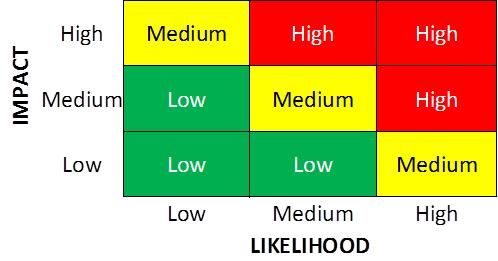
\includegraphics[scale=0.8]{Updated-Risk-Matrix.jpg} % w finalnej prezentacji może się lepiej ułoży
\end{center}


\end{document}
